%%%%%%%%%%%%%%%%%%%%%%%%%%%%%%%%%%%%%%%%%%%%%%%%%%%%%%%%%%%%%%%%%
% Qualificacao de Doutorado / Dept Fisica, CFM, UFSC            %
% Eduardo@UFSC - 2015                                           %
%%%%%%%%%%%%%%%%%%%%%%%%%%%%%%%%%%%%%%%%%%%%%%%%%%%%%%%%%%%%%%%%%

%:::::::::::::::::::::::::::::::::::::::::::::::::::::::::::::::%
%                                                               %
%                          Capítulo 2                           %
%                                                               %
%:::::::::::::::::::::::::::::::::::::::::::::::::::::::::::::::%

%***************************************************************%
%                                                               %
%                        EmLinesDataCube                        %
%                                                               %
%***************************************************************%

\chapter{Linhas de emissão}
\label{sec:emlines}

Espectros observados carregam uma mistura de luz provenientes de distintas componentes das galáxias
(estrelas, gás, poeira, etc). Com a síntese de populações estelares pode-se modelar os espectros
proveniente das estrelas de diferentes idades e composições químicas (metalicidade), além da
correção pela aplicação de uma lei de extinção por poeira. Subtraindo os espectros observados dos
espectros modelados obtêm-se os espectros residuais, compostos basicamente pelas linhas de emissão.
Essas linhas são geradas principalmente através das ionizações e recombinações de átomos dos
elementos encontrados no meio interestelar, e mais densamente, nas nuvens de gás. Neste capítulo
descrevo um módulo em \pyt que desenvolvemos para incluir medidas de linhas de emissão (e seus
subprodutos) derivados em nossa plataforma geral de análise dos cubos de dados do CALIFA.

\section{EmLinesDataCube}
\label{sec:emline:datacube}

Dentre os diversos produtos indiretos da síntese de populações estelares, a medida dos fluxos
integrados das linhas de emissão é peça fundamental em nosso projeto. Rubén García Benito, nosso
colaborador e membro no projeto CALIFA, desenvolveu um programa que, utilizando-se dos espectros
residuais  ajusta perfis gaussianos para as linhas possibilitando então a medida dos fluxos
integrados das linhas de emissão além de estimar os erros envolvidos neste processo. Um exemplo
desse processo pode ser observado na Fig.\ \ref{fig:rgbline}. Nela vemos a linha de \Hbeta na zona
central do objeto UGC00148 e o ajuste feito pelo programa. Provavelmente essas medidas sejam
liberadas para a comunidade científica assim que o último lançamento público de dados do CALIFA for
feito (DR3).

\begin{figure}
	\centering
	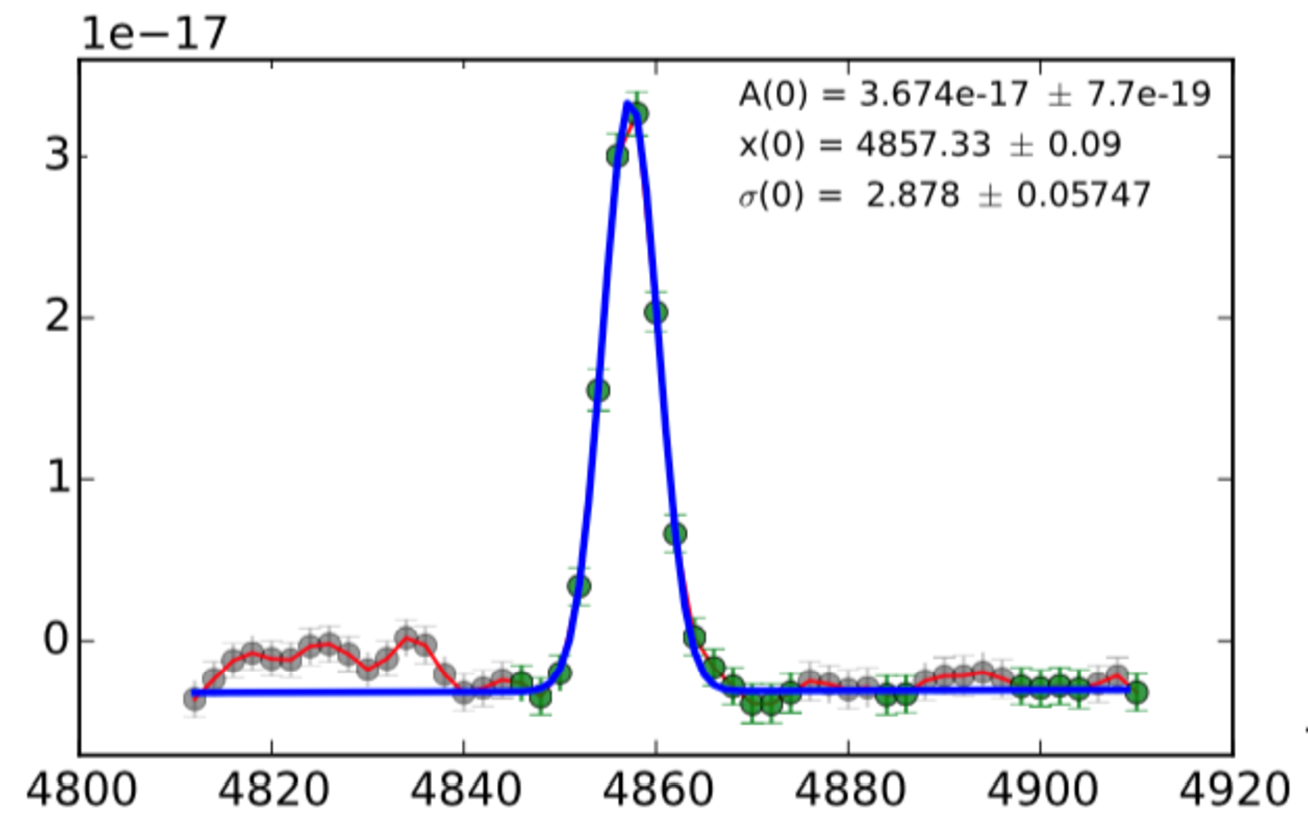
\includegraphics[scale=0.6]{figuras/K0012-zone0-Hb.pdf}
	\caption[Exemplo de ajuste de linha de emissão]
	{Espectro na região da linha de \Hbeta em emissão para a zona central da galáxia UGC00148 (objeto
CALIFA 12) juntamente com o melhor ajuste utilizando uma gaussiana. Em destaque a amplitude (A), o
comprimento de onda central (x) e o desvio padrão neste ajuste (\sigma).}
	\label{fig:rgbline}
\end{figure}

Feitas as medidas, temos o arcabouço para calcularmos várias propriedades nebulares. Escrevemos um
objeto em \pyt (cujo nome titula esta seção) que, além de organizar os resultados provenientes do
programa de medida das linhas de emissão, também calcula a abundância de oxigênio nebular, índice
que usamos como metalicidade nebular ($\log\ O/H$), o coeficiente de extinção para as regiões
nebulares ($\tauVN$), larguras equivalentes das linhas, assim como os erros propagados em cada
cálculo. Esse objeto foi adicionado ao \pycasso\footnote{{\em Python CALIFA Stellar Synthesys
Organizer} -
\href{http://minerva.ufsc.br/~andre/PyCASSO-0.9.3/intro.html}
{http://minerva.ufsc.br/$\sim$andre/PyCASSO-0.9.3/intro.html}} \citep{CidFernandes.etal.2013a} para
que os demais membros do projeto possam utilizá-lo. Nele também encontram-se as medidas dos fluxos
em diversas linhas de emissão, a posição central das linhas medidas, amplitudes, desvios padrão,
coeficientes para reconstrução do contínuo em cada linha de emissão, os erros nestas medidas, além
das propriedades mencionadas anteriormente e seus erros propagados.

\subsection{Extinção estimada através do decremento de Balmer}
\label{sec:emline:datacube:tauvneb}

Em um modelo que assume que entre o observador e a fonte de energia existe uma camada difusa, como
uma cortina, que extingue a luz diferentemente em cada comprimento de onda, temos:
\begin{equation}
	F_\lambda^{obs} = F_\lambda^{int} e^{-\tau_\lambda}
    \label{eq:extin}
\end{equation}
\noindent onde $F_\lambda^{int}$ é o fluxo intrínseco ($F_\lambda^{obs}$, o observado) em cada
comprimento de onda, $\tau_\lambda$ é a profundidade óptica para o comprimento de
onda $\lambda$ (neste trabalho também o chamamos de coeficiente de extinção). O modelo de extinção
de \citet{CCM1989a} nos dá uma calibração empírica da razão entre os coeficientes de extinção em um
comprimento de onda e na banda V, e com isso podemos desenvolver \eqref{eq:extin} de maneira que
possamos escrever uma equação para $\tau_V$:
\begin{eqnarray}
   F_\lambda^{obs} &=& F_\lambda^{int} e^{-(\frac{\tau_\lambda}{\tauV}) \tauV} \\
   q_\lambda &\equiv& \frac{\tau_\lambda}{\tauV} \\
   F_\lambda^{obs} &=& F_\lambda^{int} e^{-q_\lambda \tauV} \\
   \frac{F_\lambda^{obs}}{F_{\lambda^\prime}^{obs}} &=& \
 \frac{F_\lambda^{int} e^{-q_\lambda \tauV}}{F_{\lambda^\prime}^{int} e^{-q_{\lambda^\prime} \tauV}} \\
   \ln \left(\frac{F_\lambda^{obs}}{F_{\lambda^\prime}^{obs}}\right) &=& \
 \tauV (q_{\lambda^\prime} - q_\lambda) \ln \left(\frac{F_\lambda^{int}}{F_{\lambda^\prime}^{int}}\right) \\
   \tauV &=& \frac{1}{(q_{\lambda^\prime} - q_\lambda)} \left[\ln \ 
 \left(\frac{F_\lambda^{obs}}{F_{\lambda^\prime}^{obs}}\right) - \
 \ln \left(\frac{F_\lambda^{int}}{F_{\lambda^\prime}^{int}}\right)\right] 
 \label{eq:tauV}
\end{eqnarray}
\noindent Nessa equação, os $q_\lambda$ são provenientes da curva de extinção adotada.

Utilizando \eqref{eq:tauV} podemos calcular qual o coeficiente de extinção para essas regiões
nebulares. Para este cálculo utilizamos o fato de que a razão entre os fluxos intrínsecos das duas
primeiras linhas da série de Balmer, \Halpha e \Hbeta, varia muito um pouco com a metalicidade, a
densidade e a temperatura. Usamos aqui esse valor como constante e igual a $2.86$
\citep[densidade eletrônica de $n = 100\ cm^{-3}$ e temperatura eletrônica $T_e = 10^4$ K;
][]{Osterbrock.Ferland.2006a}. Tambem utilizamos $q_{\Halpha}  = 0.81775$ e $q_{\Hbeta} = 1.16427$
(valores da calibração empírica feita por \citeauthor{CCM1989a}). Com isso temos:
\begin{equation}
	\tauVN = 2.886\ \ln \left( \frac{F_{\Halpha}^{obs}/F_{\Hbeta}^{obs}}{2.86} \right).
\end{equation}

Como veremos mais adiante $\tauVN$ varia tipicamente entre 0.6 e 0.65 (média e mediana) nas regiões aqui
estudadas (Sec.\ \ref{sec:synvsneb:tauv} e também Fig.\ \ref{fig:HistoRadProfProps}
- {\em painel i}). O erro propagado para $\tauVN$ é:
\begin{eqnarray}
	\tauVN &\equiv& \tauVN(F_{\Halpha}^{obs}, F_{\Hbeta}^{obs}) \\
	\epsilon (\tauVN) &=& \sqrt{\left(\del{\tauVN}{F_{\Halpha}^{obs}}\right)^2 \
\epsilon (F_{\Halpha}^{obs})^2 + \left(\del{\tauVN}{F_{\Hbeta}^{obs}}\right)^2 \
\epsilon (F_{\Hbeta}^{obs})^2 } \\
	\del{\tauVN}{F_{\Halpha}^{obs}} &=& \frac{1}{F_{\Halpha}^{obs} (q_{\Hbeta} - q_{\Halpha})} \\
	\del{\tauVN}{F_{\Hbeta}^{obs}} &=& - \frac{1}{F_{\Hbeta}^{obs} (q_{\Hbeta} - q_{\Halpha})} \\
	\epsilon (\tauVN) &=& \frac{1}{(q_{\Hbeta} - q_{\Halpha})} \
\sqrt{\left(\frac{\epsilon (F_{\Halpha}^{obs})}{F_{\Halpha}^{obs}}\right)^2 + \
\left(\frac{\epsilon (F_{\Hbeta}^{obs})}{F_{\Hbeta}^{obs}}\right)^2 }
	\label{eq:etauneb}
\end{eqnarray}
\noindent Os termos de dentro da raiz em \eqref{eq:etauneb} são o inverso das relações sinal-ruído
($S/N$) de \Halpha e \Hbeta. Como \Hbeta é sempre a mais ruidosa das duas, podemos aproximar a
incerteza em $\tauVN$ por:
\begin{equation}
	\epsilon (\tauVN) \approx \frac{2.886}{(S/N)_{\Hbeta}}
	\label{eq:etaunebaprox}
\end{equation}
\noindent com valor típico \sim 0.14.

\subsection{Metalicidade Nebular}
\label{sec:emline:datacube:Zneb}

Todos os elementos, além do hidrogênio e do hélio, são considerados metais em astrofísica. O cálculo
dos indicadores de metalicidade nebular geralmente é baseado em algum método empírico indireto que
utiliza linhas fortes \citep[\emph{strong-line methods}; ][]{Pagel.etal.1979a}. Dentre estes, os
mais utilizados são aqueles que exploram razões das linhas de \OIII e \NII buscando correlações com
a abundância relativa de oxigênio nebular. Essa abundância também pode ser calculada diretamente
utilizando os coeficientes de emissão dos íons de $O$ e $H$ e medidas de algumas linhas observadas.
Esses coeficientes são dependentes da temperatura eletrônica e da densidade, que geralmente
dependem de medidas de linhas muito fracas que só podem ser observadas em regiões \Hii. As
calibrações destes indicadores de metalicidade nebular que estão sendo utilizadas pelo CALIFA foram
feitas por \citet[][M13 daqui em diante]{Marino.etal.2013a} de forma empírica utilizando medidas de
temperatura eletrônica de 603 regiões \Hii e mais medidas nebulares de 3423 regiões \Hii mapeadas
por \citet{Sanchez.etal.2013a}. O indicador que estamos utilizando para esse projeto é aquele que
calibra a fração relativa de oxigênio utilizando a razão entre as linhas de \oIII e \nII. A
parametrização encontrada pelos autores foi:
\begin{equation}
	12 + \log (O/H) = 8.533[\pm0.012] - 0.214[\pm0.012]\times \textrm{O3N2}
\end{equation}
\noindent onde O3N2 vem da razão entre os fluxos intrínsecos de \oIII, \Hbeta, \nII e \Halpha:
\begin{equation}
	\textrm{O3N2}\ \equiv\ \log \left(\frac{\OIII}{\Hbeta} \times \frac{\Halpha}{\NII}\right). 
\end{equation}
A Fig.\ \ref{fig:Marino2013_O3N2} mostra o resultado da calibração por M13. As regiões estudadas
nesse trabalho possuem abundâncias relativas de oxigênio nebular com média (mediana) $0.60\
(O/H)_\odot$ ($0.58\ (O/H)_\odot$).

\begin{figure}
	\centering
	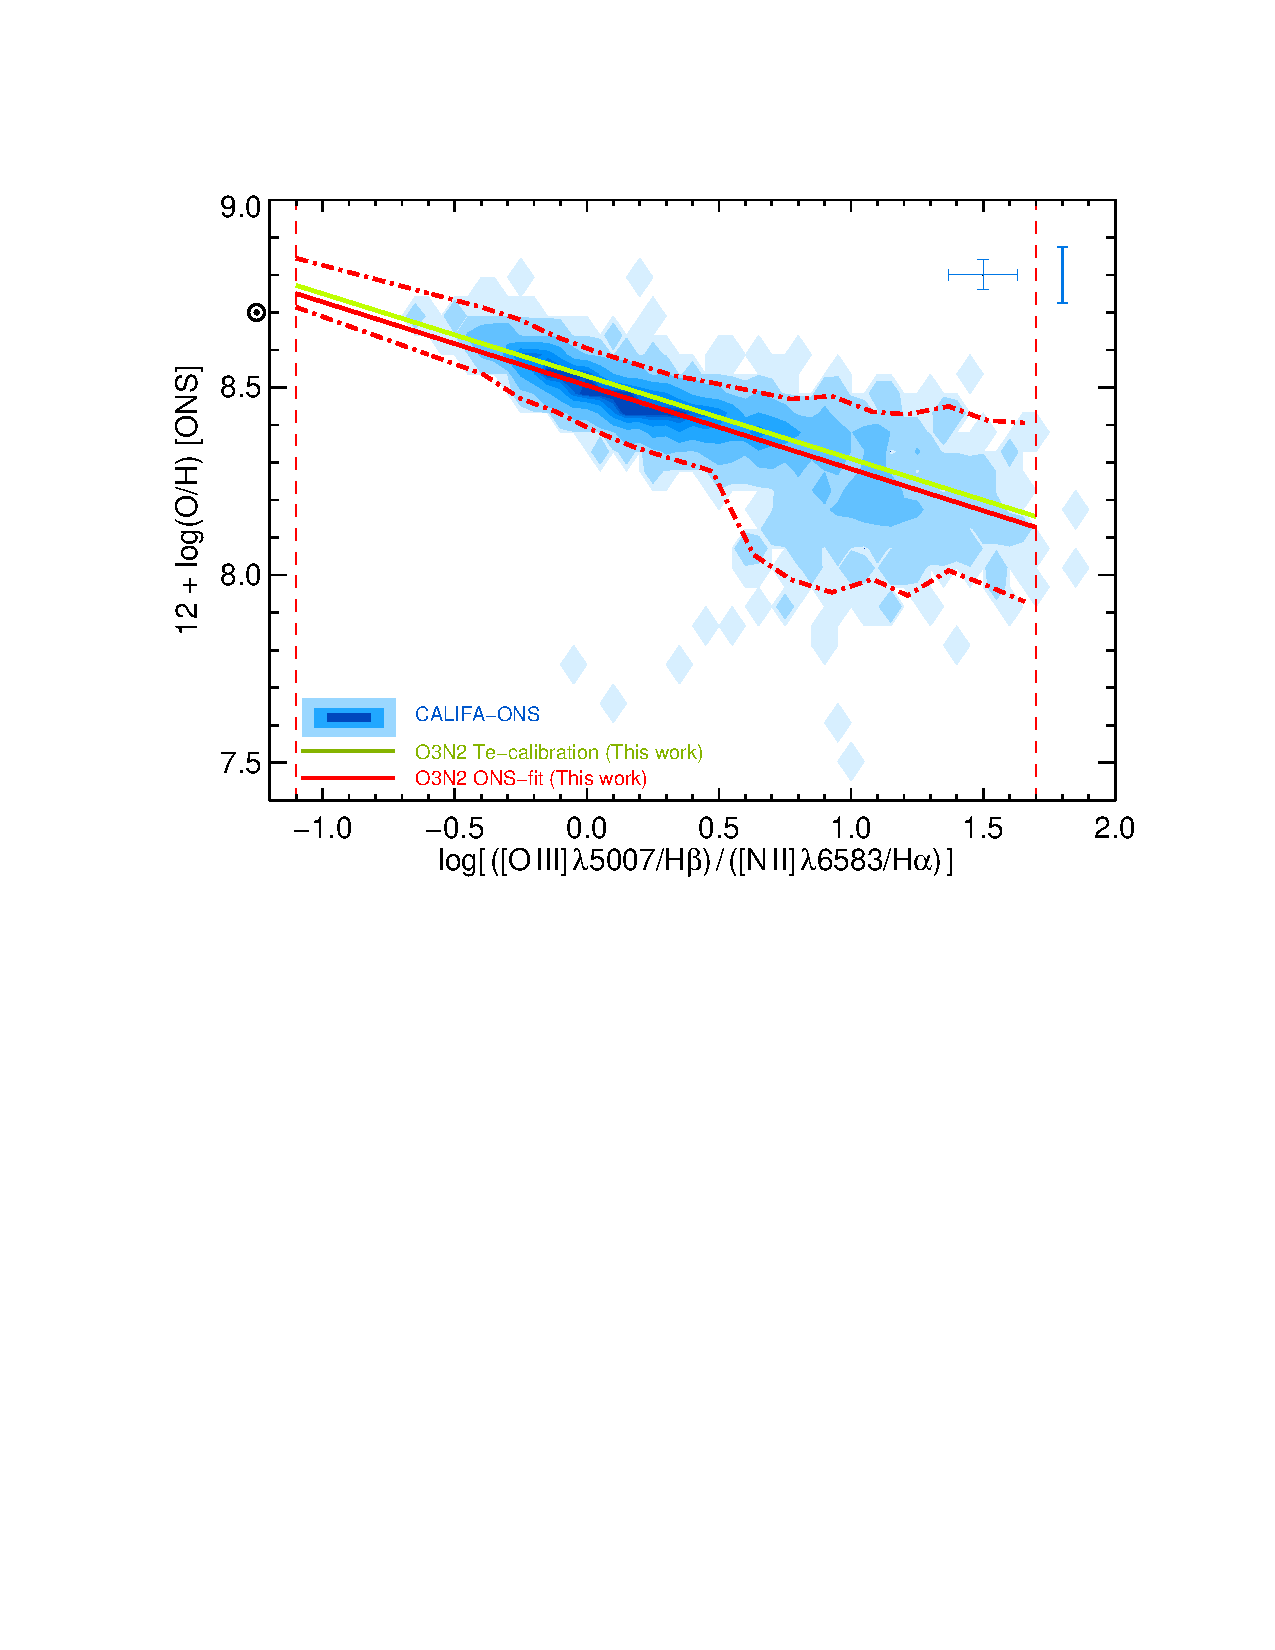
\includegraphics[scale=0.7, trim=2cm 13cm 2cm 3cm, clip]{figuras/O3N2_CALIFA.pdf}
	\caption[Calibração da abundância de oxigênio no gás]{Calibração da abundância de oxigênio 
	nebular	para 3423 regiões \Hii mapeadas por \citet{Sanchez.etal.2013a}. Figura retirada de 
	\citet{Marino.etal.2013a}}
	\label{fig:Marino2013_O3N2}
\end{figure}

\subsection{Exemplo de utilização}
\label{sec:emline:datacube:exemple}

Com a criação do objeto \emldc e sua adição ao \pycasso, o processo de análise e produção de
gráficos torna-se extremamente simples. Um exemplo de programa para produzir um gráfico BPT
\citep{Baldwin.Phillips.Terlevich.1981a} utilizando os fluxos de quatro linhas de emissão (\Halpha,
\Hbeta, \OIII e \NII) pode ser visto na Fig.\ \ref{fig:BPTprog}. Primeiro carregam-se os arquivos de
dados utilizando o \pycasso e o \emldc então todas as informações já estão prontas para serem
utilizadas. Calculam-se então as razões entre as linhas e, por último, o gráfico é feito utilizando
a biblioteca gráfica M\textsc{atplotlib} \footnote{
	\href{http://matplotlib.org/}{http://matplotlib.org/}
}.

Na Fig.\ \ref{fig:BPTfig} podemos ver uma imagem produzida por um programa como o do exemplo
anterior. Neste caso utilizamos os dados da galáxia NGC2916 (objeto CALIFA 277).
Classificada com tipo morfológico Sb, é considerad uma galáxia azul e com massa intermediária ($\sim
10^{11}\ M_\odot$). Todas as zonas neste gráfico possuem $S/N$ maior que 3 em todas as quatro linhas
do BPT (\Hbeta, \oIII, \Halpha e \nII). Podemos ver que as zonas mais próximas ao núcleo da galáxia
estão distribuídas na ponta da asa direita no plano BPT, lado associado aos núcleos ativos. Já do
outro lado do gráfico, local associado às regiões de formação estelar, se encontram as zonas
pertencentes ao disco da galáxia (R > 0.7HLR).

\begin{figure}
	\begin{python}
import numpy as np
from matplotlib import pyplot as plt
from pycasso import fitsQ3DataCube

CALIFASuperFits='K0277.fits'
EmLinesFits='K0277.EML.fits'
# Carregando arquivos FITS
K = fitsQ3DataCube(CALIFASuperFits)
K.loadEmLinesDataCube(EmLinesFits)
# Agora todos as informacoes sobre as linhas de
# emissao estao instanciadas em K.EL

# Indices dos vetores aonde estao armazenados os
# fluxos de cada linha
Ha_obs__z = K.EL.flux[K.EL.lines.index('6563'), :]
Hb_obs__z = K.EL.flux[K.EL.lines.index('4861'), :]
N2_obs__z = K.EL.flux[K.EL.lines.index('6583'), :]
O3_obs__z = K.EL.flux[K.EL.lines.index('5007'), :]
# Razao entre os fluxos de N2/Ha e O3/Hb
N2Ha__z = np.log10(N2_obs__z) - np.log10(Ha_obs__z)
O3Hb__z = np.log10(O3_obs__z) - np.log10(Hb_obs__z)

# Grafico
f = plt.figure()
ax = f.gca()
sc = ax.scatter(N2Ha__z, O3Hb__z, c = K.zoneDistance_HLR,
           		cmap = 'viridis_r', marker = 'o', s = 10, 
           		alpha = 0.8, edgecolor = 'none')
ax.set_xlabel(r'$\log\ [NII]/H\alpha$')
ax.set_ylabel(r'$\log\ [OIII]/H\beta$')
cb = plt.colorbar(sc, ticks = [0, 0.5, 1, 1.5, 2])
cb.set_label('R [HLR]')
plt.axis([-0.6, 0.3, -1.5, 1])
f.savefig('%s-BPT.pdf' % K.califaID)
	\end{python}
	\caption[Exemplo de programa utilizando o EmLinesDataCube]
	{Exemplo de programa utilizando os fluxos de \Halpha, \Hbeta, \OIII e \NII 
para construção de um gráfico BPT utilizando o objeto \emldc juntamente com o \pycasso.}
	\label{fig:BPTprog}
\end{figure}

\begin{figure}
	\centering
	%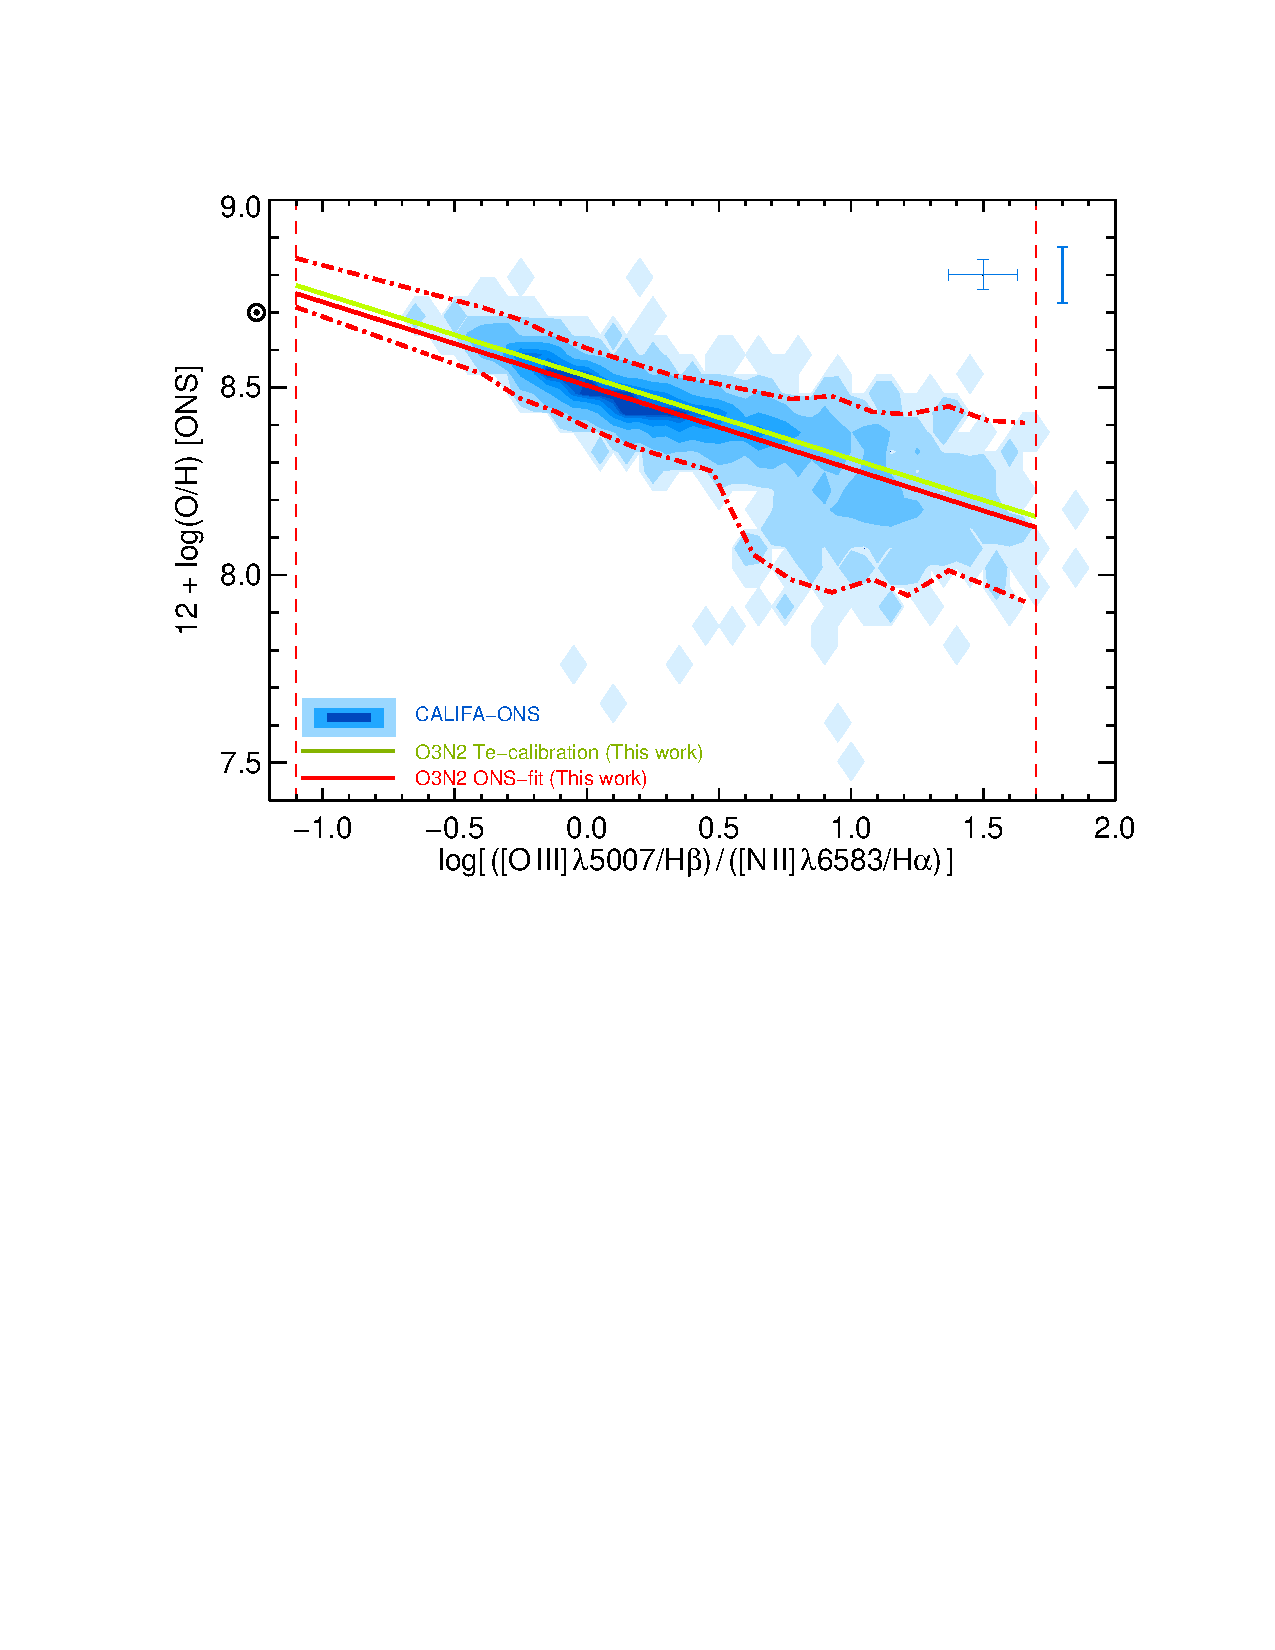
\includegraphics[scale=0.8, trim=2cm 13cm 2cm 3cm, clip]{figuras/O3N2_CALIFA.pdf}
	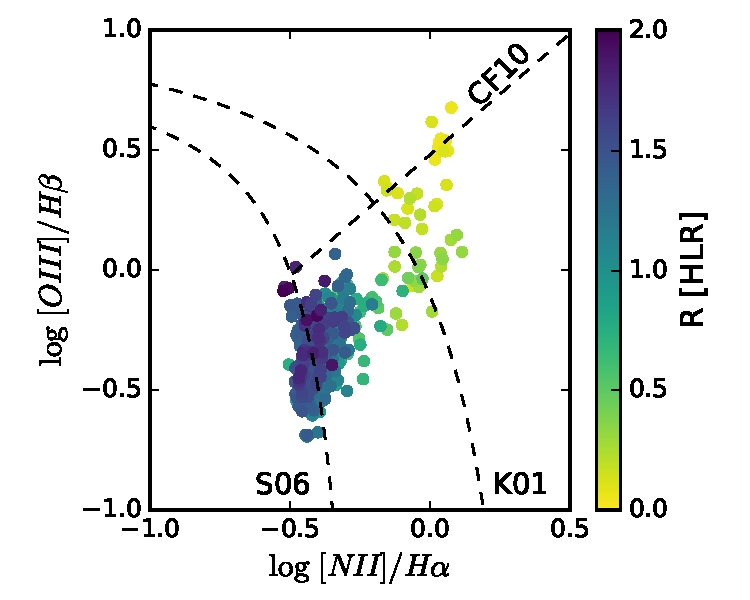
\includegraphics[scale=0.6]{figuras/K0277-BPT.pdf}
	\caption[Diagrama BPT da galáxia NGC2916]
	{Diagrama BPT para as regiões com $S/N > 3$ nas linhas \Hbeta, \OIII, \Halpha e \NII, da galáxia
NGC2916 (objeto CALIFA 277) produzida por um programa como o do exemplo da Fig.\ \ref{fig:BPTprog}.
As cores marcam a distância ao centro da galáxia em unidades do raio que contém metade da luz (HLR). As
linhas são definidas por \citet[][K01]{Kewley.etal.2001a}, \citet[][S06]{Stasinska.etal.2006a} e
\citet[][CF10]{CidFernandes.etal.2010a}.}
	\label{fig:BPTfig}
\end{figure}

\section{Taxa de formação estelar}
\label{sec:emlines:SFR}

Um dos métodos mais utilizados para medida de taxa de formação estelar ({\em Star Formation Rate} -
SFR) recente utiliza a linha de emissão de \Halpha. Nesse método assume-se que a formação estelar é
constante nos últimos $t$ anos, que deve englobar pelo menos o tempo de vida das estrelas massivas
ionizantes, que produzem basicamente todos os fótons que geram a linha de emissão de \Halpha.

Nós queremos calibrar a luminosidade da linha de \Halpha ($\LHalpha$) como um indicador
de SFR usando uma relação linear:
\begin{equation}
	\mathrm{SFR}_{\Halpha} = k \times \LHalpha.
	\label{eq:SFRHa}
\end{equation}
\noindent Portanto, nosso trabalho é encontrar $k$. Faremos isso investigando a natureza dos 
fótons H-ionizantes.

Chamamos $\Lambda$ o valor total de luz ($l$) que recebemos de estrelas que se formaram $t$ anos
atrás. $l(t)$ pode ser qualquer função que descreve a evolução temporal de qualquer fonte radiativa
genérica \emph{por unidade de massa formada} de uma população estelar simples ({\em Simple Stellar
Population} - SSP). Como depende da massa formada fica claro que essa quantidade é dependente da
Função de Massa Inicial ({\em Initial Mass Function} - IMF):
\begin{equation}
	\Lambda(t) = \int_0^t l(t')\ \textrm{d}\textrm{M}(t').
	\label{eq:dLambda}
\end{equation}
\noindent Para obter $\Lambda$ nos falta saber como a massa em estrelas cresce no tempo, ou seja,
saber como a SFR varia no tempo:
\begin{equation}
	\mathrm{d}\mathrm{M}(t)\ =\ \mathrm{SFR}(t)\ \mathrm{d}t
	\label{eq:dM_t}
\end{equation}

Utilizando \eqref{eq:dM_t} em \eqref{eq:dLambda} e integrando dentro do tempo do Universo ($T_U\
\sim$ 14 bilhões de anos) teremos hoje um total de luz:
\begin{eqnarray}
	\Lambda(t = T_U) &=& \int_0^{T_U} l(t)\ \textrm{d}\textrm{M}(t) \\
	&=& \int_0^{T_U} \mathrm{SFR}(t)\ l(t)\ \textrm{d}t
	\label{eq:Lambda}
\end{eqnarray}
\noindent Assumindo o caso B de recombinação do hidrogênio, um em cada 2.226 fótons
ionizantes produzem um fóton de \Halpha \citep{Osterbrock.Ferland.2006a}. Esse número não varia
muito em função da temperatura e da densidade nas regiões \Hii. Portanto:
\begin{equation}
	\LHalpha = h \nu_{\Halpha} \frac{\mathrm{Q}_H}{2.226},
	\label{eq:LHa_recomb_theory}
\end{equation}
\noindent onde $\mathrm{Q}_H$ é a taxa de fótons H-ionizantes. Em todo este processo assume-se que
nenhuma radiação ionizante escapa da nuvem e, apesar de $\LHalpha$ estar corrigido por
extinção, também assume-se que a poeira não absorve muito os fótons com $h\nu\ > 13.6$ eV.
Escrevemos $dQ_H$ como a equação \eqref{eq:dLambda}.
\begin{equation}
	Q_H(t)\ =\ \int dQ_H = \int q_H(t)\ \mathrm{d}\mathrm{M}(t) 
	\label{eq:QH_t}
\end{equation}
\noindent Nas equações acima, $q_H$ (que assume o mesmo papel de $l(t)$ na Eq.\ \ref{eq:dLambda}) é
a taxa de fótons H-ionizantes por unidade de massa formada. Considerando os fótons que possam ionizar
o hidrogênio ($h\nu\ \geq\ 13.6$ eV ou $\lambda\ \leq\ 912\AA$) escrevemos:
\begin{equation}
	q_H(t) = \int_0^{912\AA} \frac{l_\lambda\ \lambda}{h c} d\lambda.
	\label{eq:qH}
\end{equation}
\noindent Nesta equação, $l_\lambda$ é a luminosidade por unidade de massa formada e comprimento de
onda em unidades solares $[\textrm{L}_\odot/\AA\textrm{M}_\odot]$ para uma SSP\footnote{Apesar de
não escritas aqui, existem dependências com Z, IMF e isócronas em $l_\lambda$ (portanto, também em
$q_H$ e todos os seus produtos)}. Com isso, nós ainda precisamos analisar como a integração de
$q_H$ evolui com o tempo, para então obter a SFR. Integrando $q_H$ de hoje até $T_U$ nós
obtemos o número de fótons H-ionizantes produzidos pelas fontes que emitem a luz $l$:
\begin{equation}
	\mathcal{N}_H = \int_0^{T_U} q_H(t)\ dt
	\label{eq:Nh}
\end{equation}

Utilizamos a base de populações estelares de \citet{BC03a} com as isócronas de Padova 2000,
juntamente com a IMF de \citet{Salpeter.1955a}. Neste caso, podemos ver na Fig.\ \ref{fig:Nh_qh} a
evolução temporal de $\mathcal{N}_H$ em valores absolutos (painel superior esquerdo) e relativamente
ao total de $\mathcal{N}_H$ (painel superior direito). Em \citet[Fig. 2b]{CidFernandes.etal.2011a}
nós podemos ver a evolução temporal de $q_H$ sob todas as idades e metalicidades\footnote{Naquele
estudo, o grupo \href{http://starlight.ufsc.br}{SEAGal/\STARLIGHT} utilizou as isócronas de Padova
1994 com a IMF de \citet{Chabrier.2003a}.}. A mesma figura é reproduzida no painel inferior. É
notável que o número de fótons H-ionizantes rapidamente converge ao máximo perto de $t = 10^7$ anos.
Também fica claro que $\mathcal{N}_H$ é dependente da metalicidade, portanto o valor de $k$ em
\eqref{eq:SFRHa} também\footnote{O valor de $k$ em nossa análise varia de 2.00 até 3.13 de
acordo com a metalicidade indo de $0.02 Z_\odot@ até @1.58 Z_\odot$.}. Utilizando \eqref{eq:dM_t}
em \eqref{eq:QH_t} e com uma simplificação graças a SFR constante dentro desta escala temporal
($\mathrm{SFR}(t)\rightarrow \mathrm{SFR}$), podemos reescrever \eqref{eq:QH_t} usando
\eqref{eq:Nh}:
\begin{equation}
	Q_H = \mathrm{SFR}\ \mathcal{N}_H(t\ =\ 10^7\ \textrm{anos, IMF, Z}{}_\star).
	\label{eq:QH_converge}
\end{equation}
\noindent Substituindo \eqref{eq:QH_converge} em \eqref{eq:LHa_recomb_theory} podemos escrever:
\begin{equation}
	\mathrm{SFR}_{\Halpha} = \frac{2.226}{\mathcal{N}_H\ h \nu_{\Halpha}} \times \LHalpha
	\label{eq:SFR_theoric}
\end{equation}
\noindent Este método resulta em uma SFR recente, em termos de que usamos o valor de $\mathcal{N}_H$
para $t = 10^7$ anos. Finalmente, resolvendo \eqref{eq:SFR_theoric} encontramos o valor para $k$ em
\eqref{eq:SFRHa}:
\begin{equation}
	\mathrm{SFR}_{\Halpha}\ [\mathrm{M}_\odot\ \mathrm{yr}^{-1}] = 3.13 \times
	\left(\frac{\LHalpha}{10^8\ \mathrm{L}_\odot}\right) = 8.1 \times 10^{-42}\ \LHalpha\ [ergs\ s^{-1}]
	\label{eq:SFRNeb}
\end{equation}

Em \citet{Kennicutt.1998a} esse coeficiente é calculado utilizando diferentes modelos estelares mas
utilizando a mesma IMF. Nosso valor é bem próximo daquele obtido no artigo ($7.9 \times 10^{-42}$). 

\begin{figure}
	\centering
	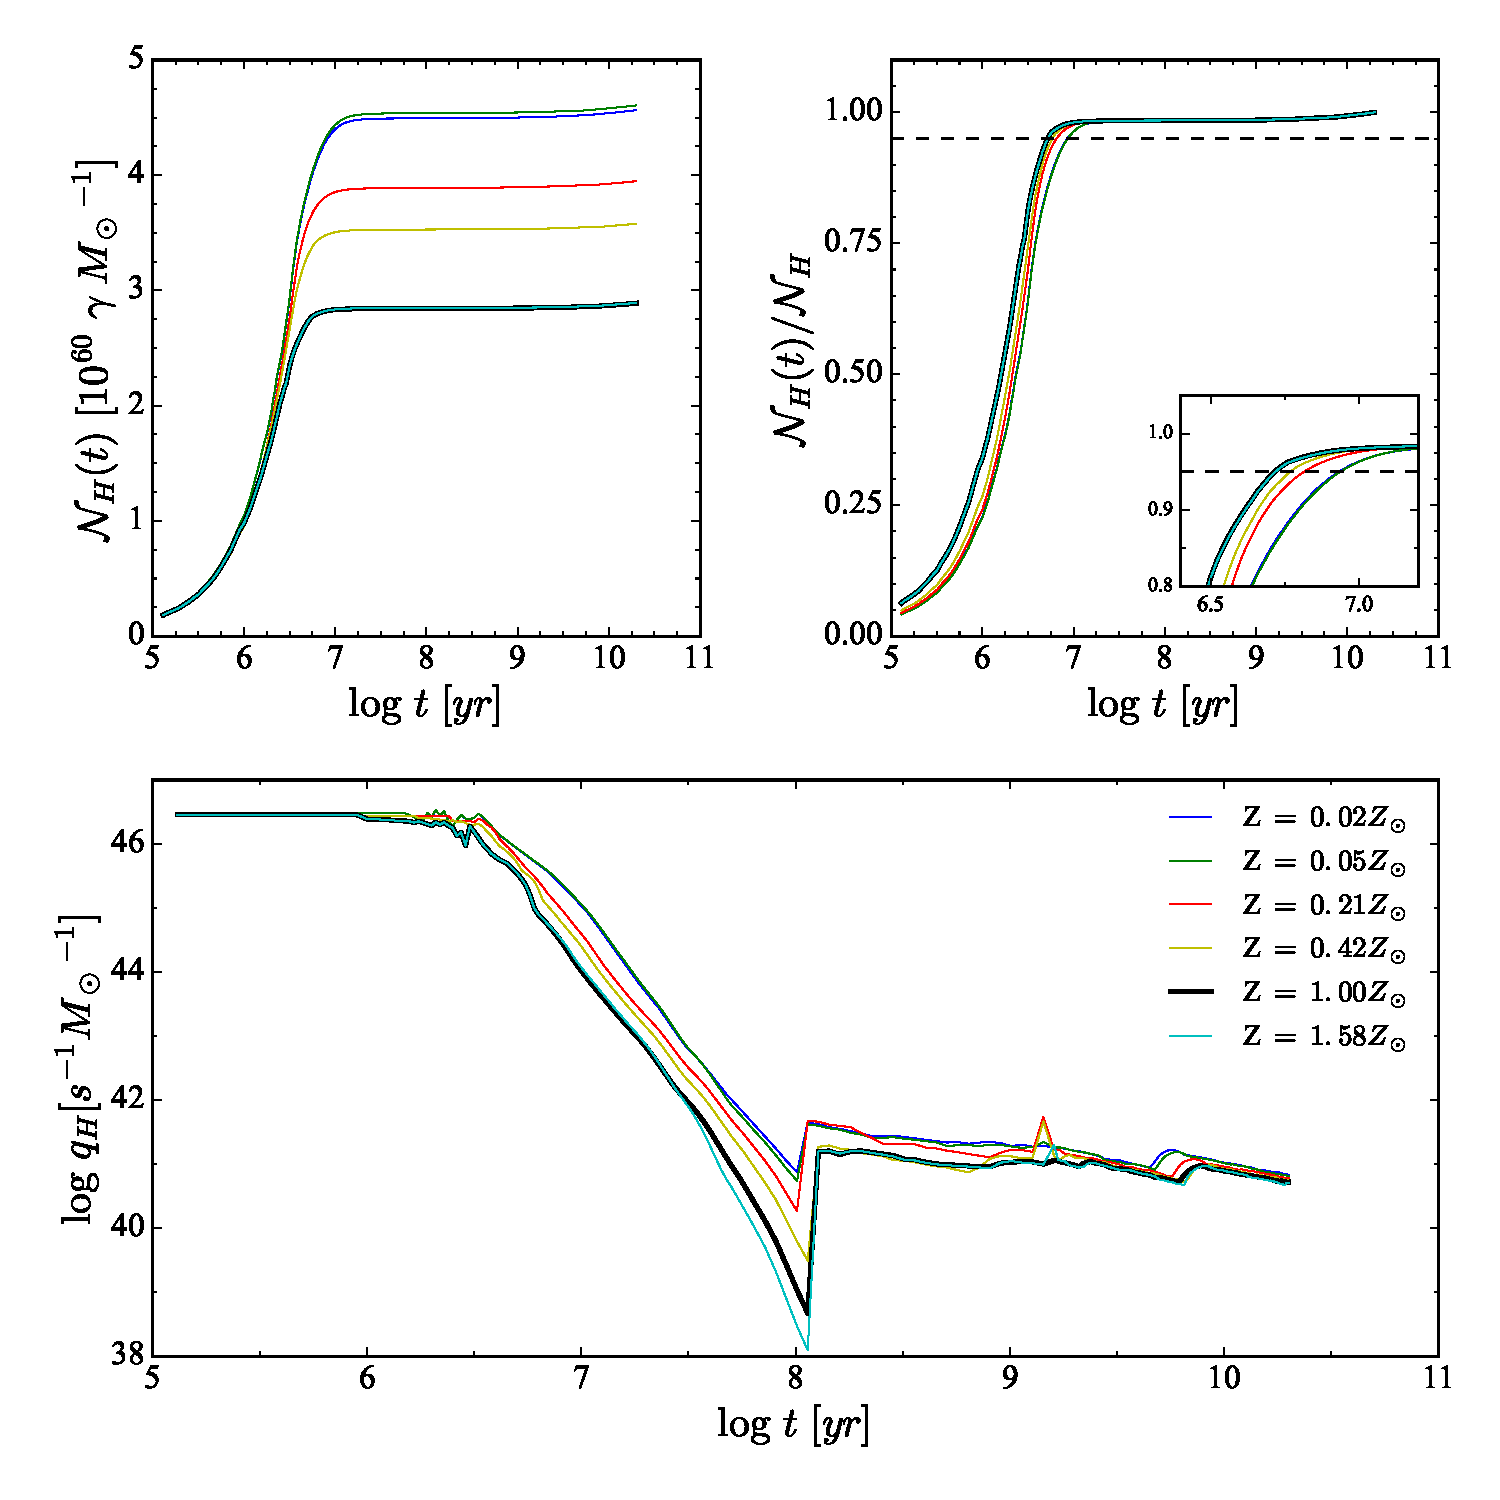
\includegraphics[scale=0.62]{figuras/Nh_logt_metBase_Padova2000_salp.pdf}
	\caption[Evolução temporal do número e da taxa de fótons H-ionizantes em unidades da massa
	formada.] 
	{\emph{Painel superior esquerdo}: A	evolução no tempo do número de fótons ($\mathcal{N}_H$) para 6
metalicidades (de 0.02 $Z_\odot$ até 1.58 $Z_\odot$) que compoem nossos modelos de SSP. A linha
preta grossa representa a evolução utilizando metalicidade solar. \emph{Painel superior direito}:
O mesmo que o \emph{painel superior esquerdo} mas normalizado pelo valor total de $\mathcal{N}_H$.
A linha pontilhada representa 95\% do total de $\mathcal{N}_H$. Em destaque a região ao redor de 10
milhões de anos. \emph{Painel inferior}: Evolução da taxa de fótons H-ionizantes em unidades da
massa formada.
Também mostra o valor seguindo o código de cores para as mesmas metalicidades.}
	\label{fig:Nh_qh}
\end{figure}
 
% End of this chapter
